% Figure 4: Confusion matrices and reliability diagrams, arms A and E.
% Generated by figures/make_fig4.py from the frozen paper_plot_packs
% (FACTS.md 8.6: F-CONF-A, F-CONF-E, F-CAL-SOURCE).
\begin{figure*}[!t]
\centering
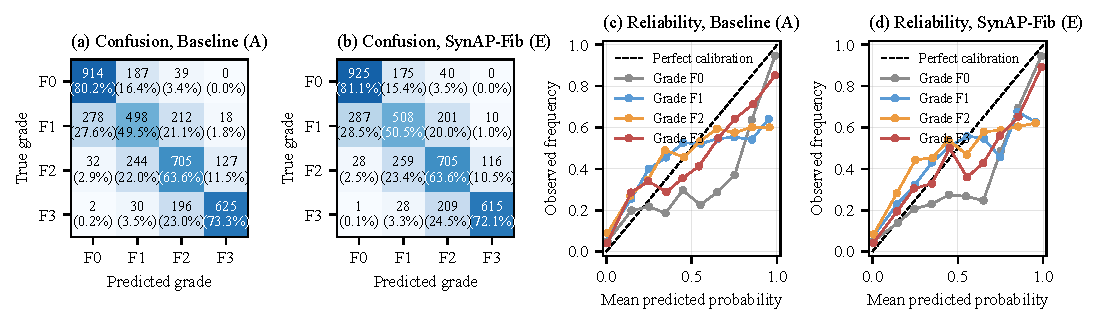
\includegraphics[width=\textwidth]{figures/fig4_confusion_calibration.pdf}
\caption{Four-grade confusion matrices (a, b) and reliability diagrams (c, d)
for the baseline (A) and SynAP-Fib (E) on the patient-held-out test set
(4,107 images; seed 2026, validation-selected checkpoints). Confusion cells
show image counts with row percentages (rows: true grade; columns: predicted
grade). Reliability diagrams plot mean predicted probability against observed
frequency for each grade, with ten probability bins per grade; the dashed
diagonal indicates perfect calibration.}
\label{fig:confcal}
\end{figure*}
